% Options for packages loaded elsewhere
\PassOptionsToPackage{unicode}{hyperref}
\PassOptionsToPackage{hyphens}{url}
\PassOptionsToPackage{dvipsnames,svgnames,x11names}{xcolor}
%
\documentclass[
  letterpaper,
  DIV=11,
  numbers=noendperiod]{scrreprt}

\usepackage{amsmath,amssymb}
\usepackage{lmodern}
\usepackage{iftex}
\ifPDFTeX
  \usepackage[T1]{fontenc}
  \usepackage[utf8]{inputenc}
  \usepackage{textcomp} % provide euro and other symbols
\else % if luatex or xetex
  \usepackage{unicode-math}
  \defaultfontfeatures{Scale=MatchLowercase}
  \defaultfontfeatures[\rmfamily]{Ligatures=TeX,Scale=1}
\fi
% Use upquote if available, for straight quotes in verbatim environments
\IfFileExists{upquote.sty}{\usepackage{upquote}}{}
\IfFileExists{microtype.sty}{% use microtype if available
  \usepackage[]{microtype}
  \UseMicrotypeSet[protrusion]{basicmath} % disable protrusion for tt fonts
}{}
\makeatletter
\@ifundefined{KOMAClassName}{% if non-KOMA class
  \IfFileExists{parskip.sty}{%
    \usepackage{parskip}
  }{% else
    \setlength{\parindent}{0pt}
    \setlength{\parskip}{6pt plus 2pt minus 1pt}}
}{% if KOMA class
  \KOMAoptions{parskip=half}}
\makeatother
\usepackage{xcolor}
\setlength{\emergencystretch}{3em} % prevent overfull lines
\setcounter{secnumdepth}{-\maxdimen} % remove section numbering
% Make \paragraph and \subparagraph free-standing
\ifx\paragraph\undefined\else
  \let\oldparagraph\paragraph
  \renewcommand{\paragraph}[1]{\oldparagraph{#1}\mbox{}}
\fi
\ifx\subparagraph\undefined\else
  \let\oldsubparagraph\subparagraph
  \renewcommand{\subparagraph}[1]{\oldsubparagraph{#1}\mbox{}}
\fi

\usepackage{color}
\usepackage{fancyvrb}
\newcommand{\VerbBar}{|}
\newcommand{\VERB}{\Verb[commandchars=\\\{\}]}
\DefineVerbatimEnvironment{Highlighting}{Verbatim}{commandchars=\\\{\}}
% Add ',fontsize=\small' for more characters per line
\usepackage{framed}
\definecolor{shadecolor}{RGB}{241,243,245}
\newenvironment{Shaded}{\begin{snugshade}}{\end{snugshade}}
\newcommand{\AlertTok}[1]{\textcolor[rgb]{0.68,0.00,0.00}{#1}}
\newcommand{\AnnotationTok}[1]{\textcolor[rgb]{0.37,0.37,0.37}{#1}}
\newcommand{\AttributeTok}[1]{\textcolor[rgb]{0.40,0.45,0.13}{#1}}
\newcommand{\BaseNTok}[1]{\textcolor[rgb]{0.68,0.00,0.00}{#1}}
\newcommand{\BuiltInTok}[1]{\textcolor[rgb]{0.00,0.23,0.31}{#1}}
\newcommand{\CharTok}[1]{\textcolor[rgb]{0.13,0.47,0.30}{#1}}
\newcommand{\CommentTok}[1]{\textcolor[rgb]{0.37,0.37,0.37}{#1}}
\newcommand{\CommentVarTok}[1]{\textcolor[rgb]{0.37,0.37,0.37}{\textit{#1}}}
\newcommand{\ConstantTok}[1]{\textcolor[rgb]{0.56,0.35,0.01}{#1}}
\newcommand{\ControlFlowTok}[1]{\textcolor[rgb]{0.00,0.23,0.31}{#1}}
\newcommand{\DataTypeTok}[1]{\textcolor[rgb]{0.68,0.00,0.00}{#1}}
\newcommand{\DecValTok}[1]{\textcolor[rgb]{0.68,0.00,0.00}{#1}}
\newcommand{\DocumentationTok}[1]{\textcolor[rgb]{0.37,0.37,0.37}{\textit{#1}}}
\newcommand{\ErrorTok}[1]{\textcolor[rgb]{0.68,0.00,0.00}{#1}}
\newcommand{\ExtensionTok}[1]{\textcolor[rgb]{0.00,0.23,0.31}{#1}}
\newcommand{\FloatTok}[1]{\textcolor[rgb]{0.68,0.00,0.00}{#1}}
\newcommand{\FunctionTok}[1]{\textcolor[rgb]{0.28,0.35,0.67}{#1}}
\newcommand{\ImportTok}[1]{\textcolor[rgb]{0.00,0.46,0.62}{#1}}
\newcommand{\InformationTok}[1]{\textcolor[rgb]{0.37,0.37,0.37}{#1}}
\newcommand{\KeywordTok}[1]{\textcolor[rgb]{0.00,0.23,0.31}{#1}}
\newcommand{\NormalTok}[1]{\textcolor[rgb]{0.00,0.23,0.31}{#1}}
\newcommand{\OperatorTok}[1]{\textcolor[rgb]{0.37,0.37,0.37}{#1}}
\newcommand{\OtherTok}[1]{\textcolor[rgb]{0.00,0.23,0.31}{#1}}
\newcommand{\PreprocessorTok}[1]{\textcolor[rgb]{0.68,0.00,0.00}{#1}}
\newcommand{\RegionMarkerTok}[1]{\textcolor[rgb]{0.00,0.23,0.31}{#1}}
\newcommand{\SpecialCharTok}[1]{\textcolor[rgb]{0.37,0.37,0.37}{#1}}
\newcommand{\SpecialStringTok}[1]{\textcolor[rgb]{0.13,0.47,0.30}{#1}}
\newcommand{\StringTok}[1]{\textcolor[rgb]{0.13,0.47,0.30}{#1}}
\newcommand{\VariableTok}[1]{\textcolor[rgb]{0.07,0.07,0.07}{#1}}
\newcommand{\VerbatimStringTok}[1]{\textcolor[rgb]{0.13,0.47,0.30}{#1}}
\newcommand{\WarningTok}[1]{\textcolor[rgb]{0.37,0.37,0.37}{\textit{#1}}}

\providecommand{\tightlist}{%
  \setlength{\itemsep}{0pt}\setlength{\parskip}{0pt}}\usepackage{longtable,booktabs,array}
\usepackage{calc} % for calculating minipage widths
% Correct order of tables after \paragraph or \subparagraph
\usepackage{etoolbox}
\makeatletter
\patchcmd\longtable{\par}{\if@noskipsec\mbox{}\fi\par}{}{}
\makeatother
% Allow footnotes in longtable head/foot
\IfFileExists{footnotehyper.sty}{\usepackage{footnotehyper}}{\usepackage{footnote}}
\makesavenoteenv{longtable}
\usepackage{graphicx}
\makeatletter
\def\maxwidth{\ifdim\Gin@nat@width>\linewidth\linewidth\else\Gin@nat@width\fi}
\def\maxheight{\ifdim\Gin@nat@height>\textheight\textheight\else\Gin@nat@height\fi}
\makeatother
% Scale images if necessary, so that they will not overflow the page
% margins by default, and it is still possible to overwrite the defaults
% using explicit options in \includegraphics[width, height, ...]{}
\setkeys{Gin}{width=\maxwidth,height=\maxheight,keepaspectratio}
% Set default figure placement to htbp
\makeatletter
\def\fps@figure{htbp}
\makeatother

\KOMAoption{captions}{tableheading}
\makeatletter
\@ifpackageloaded{tcolorbox}{}{\usepackage[many]{tcolorbox}}
\@ifpackageloaded{fontawesome5}{}{\usepackage{fontawesome5}}
\definecolor{quarto-callout-color}{HTML}{909090}
\definecolor{quarto-callout-note-color}{HTML}{0758E5}
\definecolor{quarto-callout-important-color}{HTML}{CC1914}
\definecolor{quarto-callout-warning-color}{HTML}{EB9113}
\definecolor{quarto-callout-tip-color}{HTML}{00A047}
\definecolor{quarto-callout-caution-color}{HTML}{FC5300}
\definecolor{quarto-callout-color-frame}{HTML}{acacac}
\definecolor{quarto-callout-note-color-frame}{HTML}{4582ec}
\definecolor{quarto-callout-important-color-frame}{HTML}{d9534f}
\definecolor{quarto-callout-warning-color-frame}{HTML}{f0ad4e}
\definecolor{quarto-callout-tip-color-frame}{HTML}{02b875}
\definecolor{quarto-callout-caution-color-frame}{HTML}{fd7e14}
\makeatother
\makeatletter
\makeatother
\makeatletter
\makeatother
\makeatletter
\@ifpackageloaded{caption}{}{\usepackage{caption}}
\AtBeginDocument{%
\ifdefined\contentsname
  \renewcommand*\contentsname{Table of contents}
\else
  \newcommand\contentsname{Table of contents}
\fi
\ifdefined\listfigurename
  \renewcommand*\listfigurename{List of Figures}
\else
  \newcommand\listfigurename{List of Figures}
\fi
\ifdefined\listtablename
  \renewcommand*\listtablename{List of Tables}
\else
  \newcommand\listtablename{List of Tables}
\fi
\ifdefined\figurename
  \renewcommand*\figurename{Figure}
\else
  \newcommand\figurename{Figure}
\fi
\ifdefined\tablename
  \renewcommand*\tablename{Table}
\else
  \newcommand\tablename{Table}
\fi
}
\@ifpackageloaded{float}{}{\usepackage{float}}
\floatstyle{ruled}
\@ifundefined{c@chapter}{\newfloat{codelisting}{h}{lop}}{\newfloat{codelisting}{h}{lop}[chapter]}
\floatname{codelisting}{Listing}
\newcommand*\listoflistings{\listof{codelisting}{List of Listings}}
\makeatother
\makeatletter
\@ifpackageloaded{caption}{}{\usepackage{caption}}
\@ifpackageloaded{subcaption}{}{\usepackage{subcaption}}
\makeatother
\makeatletter
\@ifpackageloaded{tcolorbox}{}{\usepackage[many]{tcolorbox}}
\makeatother
\makeatletter
\@ifundefined{shadecolor}{\definecolor{shadecolor}{rgb}{.97, .97, .97}}
\makeatother
\makeatletter
\makeatother
\ifLuaTeX
  \usepackage{selnolig}  % disable illegal ligatures
\fi
\IfFileExists{bookmark.sty}{\usepackage{bookmark}}{\usepackage{hyperref}}
\IfFileExists{xurl.sty}{\usepackage{xurl}}{} % add URL line breaks if available
\urlstyle{same} % disable monospaced font for URLs
\hypersetup{
  pdftitle={First Ticket},
  colorlinks=true,
  linkcolor={blue},
  filecolor={Maroon},
  citecolor={Blue},
  urlcolor={Blue},
  pdfcreator={LaTeX via pandoc}}

\title{First Ticket}
\author{}
\date{}

\begin{document}
\maketitle
\ifdefined\Shaded\renewenvironment{Shaded}{\begin{tcolorbox}[borderline west={3pt}{0pt}{shadecolor}, frame hidden, enhanced, interior hidden, breakable, sharp corners, boxrule=0pt]}{\end{tcolorbox}}\fi

After completing the previous chapters, Daphne or Jeanette will assign a
ticket from RT. Login using your LDAP credentials got get familiarized
with RT.

\hypertarget{navigate-rt}{%
\section{Navigate RT}\label{navigate-rt}}

The RT ticketing system is how we communicate with folks interacting
with the Arctic Data Center.\\
We use it for managing submissions, accessing issues, etc. It consists
of three separate interfaces:\\
\protect\hyperlink{front-page}{Front Page}\\
\protect\hyperlink{all-tickets}{All Tickets}\\
\protect\hyperlink{example-ticket}{Ticket Page}

\hypertarget{front-page}{%
\subsection{Front page}\label{front-page}}

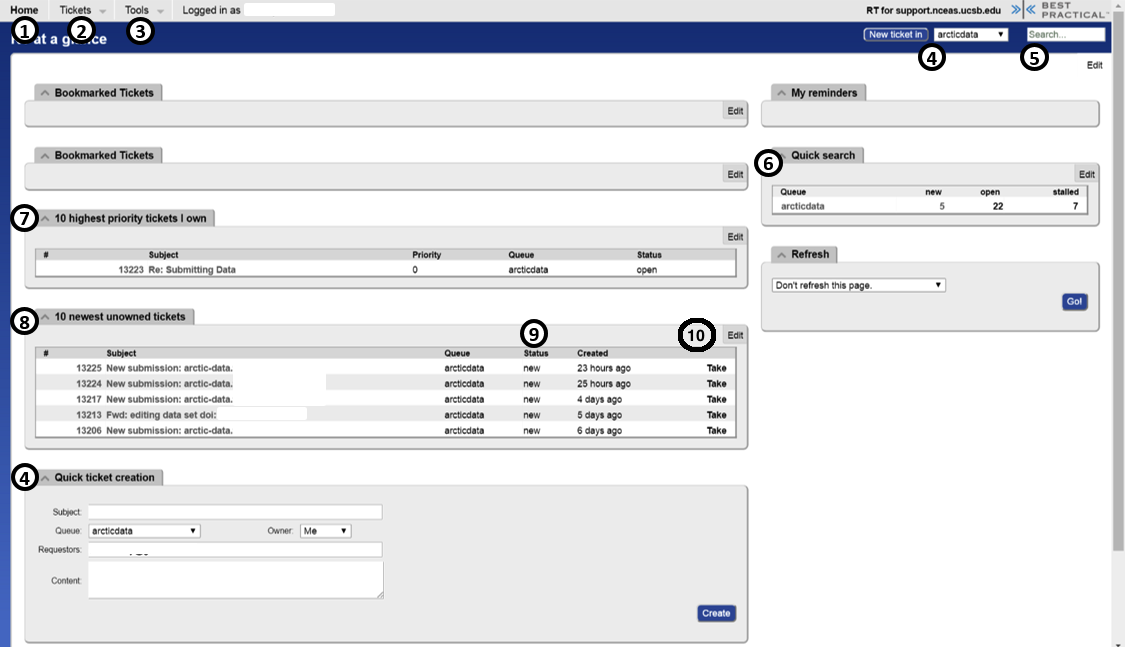
\includegraphics{../images/front_page_rt.png}

This is what you see first

\begin{enumerate}
\def\labelenumi{\arabic{enumi}.}
\tightlist
\item
  Home - brings you to this homepage\\
\item
  Tickets - to search for tickets (also see number 5)\\
\item
  Tools - not needed\\
\item
  New Ticket - create a new ticket\\
\item
  Search - Type in the ticket number to quickly navigate to a ticket\\
\item
  Queue - Lists all of the tickets currently in a particular queue (such
  as `arcticdata') and their statuses\\
\end{enumerate}

\begin{itemize}
\tightlist
\item
  New = unopened tickets that require attention\\
\item
  Open = tickets currently open and under investigation and/or being
  processed by a support team member\\
\item
  Stalled = tickets awaiting responses from the PI/ \texttt{submitter}\\
\end{itemize}

\begin{enumerate}
\def\labelenumi{\arabic{enumi}.}
\setcounter{enumi}{6}
\tightlist
\item
  Tickets I Own - These are the current open tickets that are claimed by
  me\\
\item
  Unowned Tickets - Newest tickets awaiting claim\\
\item
  Ticket Status - Status and how long ago it was created\\
\item
  Take - claim the ticket as yours
\end{enumerate}

\hypertarget{all-tickets}{%
\subsection{All tickets}\label{all-tickets}}

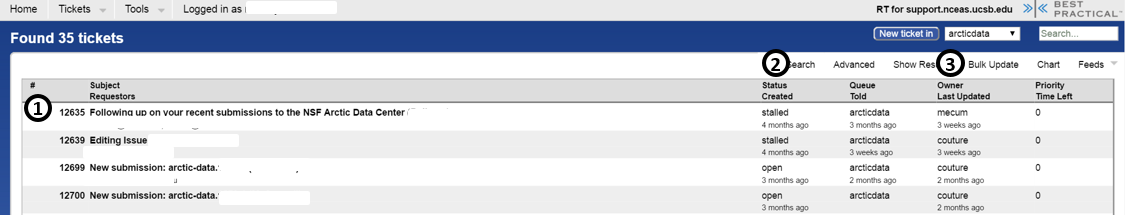
\includegraphics{../images/all_tickets_rt.png}

This is the queue interface from number 6 of the Front page\\
1. Ticket number and title\\
2. Ticket status\\
3. Owner - who has claimed the ticket

\hypertarget{example-ticket}{%
\subsection{Example ticket}\label{example-ticket}}

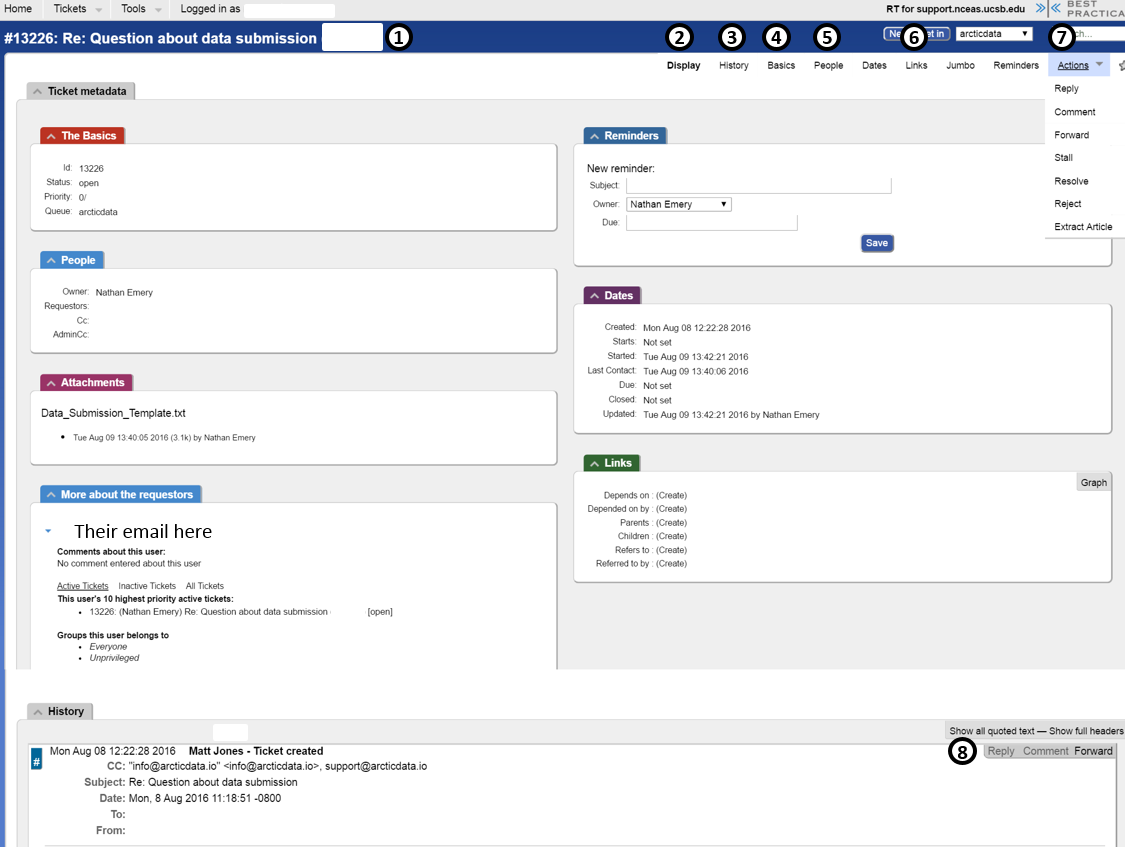
\includegraphics{../images/example_ticket_rt.png}

\begin{enumerate}
\def\labelenumi{\arabic{enumi}.}
\tightlist
\item
  Title - Include the PI's name for reference\\
\item
  Display - homepage of the ticket\\
\item
  History - Comment/Email history, see bottom of Display page\\
\item
  Basics - edit the title, status, and ownership here\\
\item
  People - option to add more people to the watch list for a given
  ticket conversation. Note that user/ PI/ \texttt{submitter} email
  addresses should be listed as ``Requestors''. Requestors are only
  emailed on ``Replys'', not ``Comments''. Ensure your ticket has a
  Requestor before attempting to contact users/ PIs/
  \texttt{submitter}s\\
\item
  Links - option to ``Merge into'' another ticket number if this is part
  of a larger conversation. Also option to add a reference to another
  ticket number
\end{enumerate}

\begin{tcolorbox}[enhanced jigsaw, arc=.35mm, toprule=.15mm, opacityback=0, colbacktitle=quarto-callout-warning-color!10!white, colframe=quarto-callout-warning-color-frame, toptitle=1mm, rightrule=.15mm, title=\textcolor{quarto-callout-warning-color}{\faExclamationTriangle}\hspace{0.5em}{Warning}, coltitle=black, bottomtitle=1mm, bottomrule=.15mm, titlerule=0mm, left=2mm, opacitybacktitle=0.6, breakable, leftrule=.75mm, colback=white]
Verify that this is indeed the two tickets you want to merge. It is
non-reversible.
\end{tcolorbox}

\begin{enumerate}
\def\labelenumi{\arabic{enumi}.}
\setcounter{enumi}{6}
\tightlist
\item
  Actions\\
\end{enumerate}

\begin{itemize}
\tightlist
\item
  Reply - message the \texttt{submitter}/ PI/ all watchers\\
\item
  Comment - attach internal message (no \texttt{submitter}s, only Data
  Teamers)\\
\item
  Open It - Open the ticket\\
\item
  Stall - \texttt{submitter} has not responded in greater than 1 month\\
\item
  Resolve - ticket completed\\
\end{itemize}

\begin{enumerate}
\def\labelenumi{\arabic{enumi}.}
\setcounter{enumi}{7}
\tightlist
\item
  History - message history and option to reply (to \texttt{submitter}
  and beyond) or comment (internal message)
\end{enumerate}

\hypertarget{new-data-submission}{%
\subsection{New data submission}\label{new-data-submission}}

When notified by Arcticbot about a new data submission, here are the
typical steps:

\begin{enumerate}
\def\labelenumi{\arabic{enumi}.}
\tightlist
\item
  Update the Requestor under the People section based on the email given
  in the submission (usually the user/ PI/ \texttt{submitter}). You may
  have to google for the e-mail address if the PI did not include it in
  the metadata record.
\item
  Take the ticket (Actions \textgreater{} Take)
\item
  Review the submission based on the checklist
\item
  Draft an email using the template and let others review it via Slack
\item
  Send your reply via Actions
\end{enumerate}

Before opening a R script first look over the initial checklist first to
identify what you will need to update in the metadata.

\hypertarget{initial-review-checklist}{%
\section{Initial review checklist}\label{initial-review-checklist}}

Before responding to a new submission use this checklist to review the
submission. When your are ready to respond use the initial email
template and insert comments and modify as needed.

\hypertarget{sensitive-data}{%
\subsubsection{Sensitive Data}\label{sensitive-data}}

If any of the below is in the dataset, please alert the \#arctica team
know before proceeding.

\begin{itemize}
\tightlist
\item
  Check if there is any sensitive information or personal identifying
  information in the data (eg. Names)
\item
  Can the data be disaggregated and de-anonymized? (eg. a small sample
  size and individuals could be easily identified by their answers)
\item
  \href{https://datadryad.org/docs/HumanSubjectsData.pdf}{Dryad Human
  Subject data guidelines} can be a good place to start
\end{itemize}

Common Cases:

\begin{itemize}
\tightlist
\item
  \textbf{Social Science:} Any dataset involving human subjects (may
  include awards awarded by ASSP and topics such as COVID-19)
\item
  \textbf{Archaeology:} archaeological site location information, which
  is protected from public access by law
\item
  \textbf{Biology:} protected species location coordinates
\end{itemize}

\hypertarget{data-citations}{%
\subsubsection{Data citations}\label{data-citations}}

\begin{itemize}
\tightlist
\item
  If the dataset appears to be in a publication please (might be in the
  abstract) make sure that those citations are registered.
\end{itemize}

\hypertarget{title}{%
\subsubsection{Title}\label{title}}

\begin{itemize}
\tightlist
\item
  WHAT, WHERE, and WHEN:

  \begin{itemize}
  \tightlist
  \item
    Is descriptive of the work (provides enough information to
    understand the contents at a general scientific level), AND includes
    temporal coverage
  \item
    Provides a location of the work from the local to state or country
    level
  \item
    Provides a time frame of the work
  \item
    NO UNDEFINED ACRONYMS, ABBREVIATIONS, nor INITIALISMS unless
    approved of as being more widely-known in that form than spelled out
  \end{itemize}
\end{itemize}

\hypertarget{abstract}{%
\subsubsection{Abstract}\label{abstract}}

\begin{itemize}
\tightlist
\item
  Describes the DATA as well as:

  \begin{itemize}
  \item
    The motivation (purpose) of the study
  \item
    Where and when the research took place
  \item
    At least one sentence summarizing general methodologies
  \item
    NO UNDEFINED ACRONYMS, ABBREVIATIONS, nor INITIALISMS unless
    approved of as being more widely-known in that form than spelled out
  \item
    At least 100 words total
  \item
    \begin{itemize}
    \tightlist
    \item
      tags such as
      \texttt{\textless{}superscript\textgreater{}2\textless{}/superscript\textgreater{}}
      and
      \texttt{\textless{}subscript\textgreater{}2\textless{}/subscript\textgreater{}}
      can be used for nicer formatting
    \end{itemize}
  \item
    Any citations to papers can be registered with us
  \end{itemize}
\end{itemize}

\hypertarget{keywords}{%
\subsubsection{Keywords}\label{keywords}}

\begin{itemize}
\tightlist
\item
  Some keywords are included
\end{itemize}

\hypertarget{data}{%
\subsubsection{Data}\label{data}}

\begin{itemize}
\tightlist
\item
  Data is normalized (if not suggest to convert the data if possible)
\item
  At least one data file, or an identifier to the files at another
  approved archive, unless funded by ASSP (Arctic Social Sciences
  Program)
\item
  No xls/xlsx files (or other proprietary files)
\item
  File contents and relationships among files are clear
\item
  Each file is well NAMED and DESCRIBED and clearly differentiated from
  all others
\item
  All attributes in EML match attribute names in respective data files
  EXACTLY, are clearly defined, have appropriate units, and are in the
  same order as in the file. Quality control all \texttt{dimensionless}
  units.
\item
  Missing value codes are explained (WHY are the data absent?)
\item
  If it is a \texttt{.rar} file -\textgreater{} scan the file
\item
  If there is the unit tons make sure to ask if it is metric tons or
  imperical tons if not clarified already
\end{itemize}

\hypertarget{people-parties}{%
\subsubsection{People \& Parties}\label{people-parties}}

\begin{itemize}
\tightlist
\item
  At least one contact and one creator with a name, email address, and
  ORCID iD
\end{itemize}

\hypertarget{coverages}{%
\subsubsection{Coverages}\label{coverages}}

\begin{itemize}
\tightlist
\item
  Includes coverages that make sense

  \begin{itemize}
  \tightlist
  \item
    Temporal coverage - Start date BEFORE end date
  \item
    Geologic time scales are added if mentioned in metadata (e.g.~8
    Million Years or a name of a time period like Jurassic)
  \item
    Spatial coverage matches geographic description (check hemispheres)
  \item
    Geographic description is from the local to state or country level,
    at the least
  \item
    Taxonomic coverage if appropriate
  \end{itemize}
\end{itemize}

\hypertarget{project-information}{%
\subsubsection{Project Information}\label{project-information}}

\begin{itemize}
\tightlist
\item
  At least one FUNDING number
\item
  Title, personnel, and abstract match information from the AWARD (not
  from the data package)
\end{itemize}

\hypertarget{methods}{%
\subsubsection{Methods}\label{methods}}

\begin{itemize}
\tightlist
\item
  This section is REQUIRED for ALL NSF-FUNDED data packages
\item
  Enough detail is provided such that a reasonable scientist could
  interpret the study and data for reuse without needing to consult the
  researchers, nor any other resources
\end{itemize}

\hypertarget{portals}{%
\subsubsection{Portals}\label{portals}}

\begin{itemize}
\tightlist
\item
  If there are multiple submissions from the same people/project let
  them know about the portals feature
\item
  If this is part of a portal make sure this dataset can be found there.
  Additional steps might be needed to get that to work. Please consult
  Jeanette and see the
  \href{https://nceas.github.io/datateam-training/reference/data-portals-1.html}{data
  portals} section.
\end{itemize}

\hypertarget{processing-templates}{%
\section{Processing templates}\label{processing-templates}}

We have developed some partially filled R scripts to get you started on
working on your first dataset. They outline common functions used in
processing a dataset. However, it will differ depending on the dataset.

You can use this template where you can
\href{data/dataset_processing_example_blanks.R}{fill in the blanks} to
get familiar with the functions we use and workflow at first. We also
have a more minimal example
\href{data/dataset_processing_example_skeleton.R}{A filled example} as a
intermediate step. You can look at the
\href{data/dataset_processing_example_filled.R}{filled example} if you
get stuck or message the \#datateam.

Once you have updated the dataset to your satisfaction and reviewed the
Final Checklist, post the link to the dataset on \#datateam for peer
review.

\hypertarget{final-checklist}{%
\section{Final Checklist}\label{final-checklist}}

You can click on the \texttt{assessment\ report} on the website to for a
general check. Fix anything you see there.

Send the link over slack for peer review by your fellow datateam
members. Usually we look for the following (the list is not exhaustive):

\hypertarget{special-datasets}{%
\subsection{Special Datasets}\label{special-datasets}}

Please refer to the dedicated pages for instructions to handle these
cases:

\begin{itemize}
\tightlist
\item
  \href{https://nceas.github.io/datateam-training/reference/MOSAiC.html}{MOSAiC}
\item
  \href{https://nceas.github.io/datateam-training/reference/distributed-biological-observatory-dbo-submissions.html}{DBO}
\end{itemize}

\hypertarget{system-metadata}{%
\subsection{System Metadata}\label{system-metadata}}

The format ids are correct

\hypertarget{general-eml}{%
\subsection{General EML}\label{general-eml}}

Included lines for FAIR:

\begin{Shaded}
\begin{Highlighting}[]
\NormalTok{doc }\OtherTok{\textless{}{-}} \FunctionTok{eml\_add\_publisher}\NormalTok{(doc)}
\NormalTok{doc }\OtherTok{\textless{}{-}} \FunctionTok{eml\_add\_entity\_system}\NormalTok{(doc)}
\end{Highlighting}
\end{Shaded}

\hypertarget{title-1}{%
\subsection{Title}\label{title-1}}

\begin{itemize}
\tightlist
\item
  No abbreviations, should include geographic and temporal coverage
\end{itemize}

\hypertarget{abstract-1}{%
\subsection{Abstract}\label{abstract-1}}

\begin{itemize}
\tightlist
\item
  longer than 100 words
\item
  no abbreviations or garbled text
\item
  tags such as
  \texttt{\textless{}superscript\textgreater{}2\textless{}/superscript\textgreater{}}
  and
  \texttt{\textless{}subscript\textgreater{}2\textless{}/subscript\textgreater{}}
  can be used for nicer formatting
\end{itemize}

\hypertarget{datatable-otherentity-spatialvectors}{%
\subsection{DataTable / OtherEntity /
SpatialVectors}\label{datatable-otherentity-spatialvectors}}

\begin{itemize}
\tightlist
\item
  in the correct one: \textbf{DataTable / OtherEntity / SpatialVector /
  SpatialRaster} for the file type
\item
  \textbf{entityDescription} - longer than 5 words and unique
\item
  \textbf{physical} present and format correct
\end{itemize}

\hypertarget{attribute-table}{%
\subsubsection{Attribute Table}\label{attribute-table}}

\begin{itemize}
\tightlist
\item
  complete
\item
  attributeDefinitions longer than 3 words
\item
  \textbf{Variables} match what is in the file
\item
  \textbf{Measurement domain} - if appropirate (ie dateTime correct)
\item
  \textbf{Missing Value Code} - accounted for if applicable
\item
  \textbf{Semantic Annotation} - appropriate semantic annotations added,
  especially for spatial and temporal variables: lat, lon, date etc.
\end{itemize}

\hypertarget{people}{%
\subsection{People}\label{people}}

\begin{itemize}
\tightlist
\item
  complete information for each person in each section

  \begin{itemize}
  \tightlist
  \item
    including ORCID and e-mail address for all contacts
  \item
    people repeated across sections should have consistent information
  \end{itemize}
\end{itemize}

\hypertarget{geographic-region}{%
\subsection{Geographic region}\label{geographic-region}}

\begin{itemize}
\tightlist
\item
  the map looks correctand matches the geographic description
\item
  check if negatives (-) are missing
\end{itemize}

\hypertarget{project}{%
\subsection{Project}\label{project}}

\begin{itemize}
\tightlist
\item
  if it is an NSF award you can use the helper function:

  \begin{itemize}
  \tightlist
  \item
    \texttt{doc\$dataset\$project\ \textless{}-\ eml\_nsf\_to\_project(awards)}
  \end{itemize}
\item
  for other awards that need to be set manually, see the
  \href{https://nceas.github.io/datateam-training/reference/set-the-project-section.html}{set
  project} page
\end{itemize}

\hypertarget{methods-1}{%
\subsection{Methods}\label{methods-1}}

\begin{itemize}
\tightlist
\item
  present
\item
  no garbled text
\end{itemize}

\hypertarget{check-eml-version}{%
\subsection{Check EML Version}\label{check-eml-version}}

\begin{itemize}
\tightlist
\item
  currently using: \texttt{eml-2.2.0} (as of July 30 2020)
\item
  review to see if the EML version is set correctly by reviewing the
  \texttt{doc\$\textasciigrave{}@context\textasciigrave{}} that it is
  indeed 2.2.0 under eml
\item
  Re-run your code again and have the
  line\texttt{emld::eml\_version("eml-2.2.0")} at the top
\item
  Make sure the system metadata is also 2.2.0
\end{itemize}

\hypertarget{access}{%
\subsection{Access}\label{access}}

\begin{itemize}
\tightlist
\item
  Granted access to PI using \texttt{set\_rights\_and\_access()}

  \begin{itemize}
  \tightlist
  \item
    make sure it is \texttt{http://} (no s)
  \end{itemize}
\item
  \textbf{note} if it is a part of portals there might be specific
  access requirements for it to be visible using \texttt{set\_access()}
\end{itemize}

\hypertarget{sftp-files}{%
\subsection{SFTP Files}\label{sftp-files}}

\begin{itemize}
\tightlist
\item
  if there are files transferred to us via SFTP, delete those files when
  the ticket is resolved
\end{itemize}

\hypertarget{updated-datasets}{%
\subsection{Updated datasets}\label{updated-datasets}}

All the above applies. These are some areas to do a closer check when
users update with a new file:

\begin{itemize}
\tightlist
\item
  New data was added

  \begin{itemize}
  \tightlist
  \item
    Temporal Coverage and Title
  \item
    and follow usual protocols
  \end{itemize}
\item
  Files were replaced

  \begin{itemize}
  \tightlist
  \item
    update physical and entityName
  \item
    double-check attributes are the same
  \item
    check for any new missing value codes that should be accounted for
  \end{itemize}
\item
  Was the dataset published before 2021?

  \begin{itemize}
  \tightlist
  \item
    update project info , annotations
  \end{itemize}
\item
  Glance over entire page for any small mistakes (ie. repeated
  additionalMetadata, any missed \&amps, typos)
\end{itemize}

After all the revisions send the link to the PI in an email through RT.
Send the draft of the email to Daphne or Jeanette on Slack.

\hypertarget{email-templates}{%
\section{Email templates}\label{email-templates}}

This section covers new data packages submitted. For other inquiries see
the PI FAQ templates

Please think critically when using these canned replies rather than just
blindly sending them. Typically, content should be adjusted/ customized
for each response to be as relevant, complete, and precise as possible.

In your first few months, please run email drafts by the \#datateam
Slack and get approval before sending.

Remember to consult the submission guidelines for details of what is
expected.

Quick reference:

\begin{itemize}
\tightlist
\item
  \href{https://nceas.github.io/datateam-training/reference/email-templates.html\#initial-email-template}{Initial
  email template}
\item
  \href{https://nceas.github.io/datateam-training/reference/email-templates.html\#final-email-templates}{Final
  email templates}
\item
  \href{https://nceas.github.io/datateam-training/reference/email-templates.html\#additional-email-templates}{Additional
  email template}
\end{itemize}

Once the dataset is approved by the PI and there are no further changes,
publish the dataset with a doi.

\begin{Shaded}
\begin{Highlighting}[]
\NormalTok{doi }\OtherTok{\textless{}{-}}\NormalTok{ dataone}\SpecialCharTok{::}\FunctionTok{generateIdentifier}\NormalTok{(d1c\_test}\SpecialCharTok{@}\NormalTok{mn, }\StringTok{"DOI"}\NormalTok{)}
\NormalTok{dp }\OtherTok{\textless{}{-}} \FunctionTok{replaceMember}\NormalTok{(dp, metadataId, }\AttributeTok{replacement =}\NormalTok{ eml\_path, }\AttributeTok{newId =}\NormalTok{ doi)}

\NormalTok{newPackageId }\OtherTok{\textless{}{-}} \FunctionTok{uploadDataPackage}\NormalTok{(d1c\_test, dp, }\AttributeTok{public =} \ConstantTok{TRUE}\NormalTok{, }\AttributeTok{quiet =} \ConstantTok{FALSE}\NormalTok{)}
\end{Highlighting}
\end{Shaded}

\hypertarget{categorize-datasets}{%
\section{Categorize datasets}\label{categorize-datasets}}

As a final step we will categorize the dataset you processed. We are
trying to categorize datasets so we can have a rough idea of what kinds
of datasets we have at the Arctic Data Center. We will grant you access
to the google sheet that has all of the
\href{https://docs.google.com/spreadsheets/d/1S_7iW0UBZLZoJBrHXTW5fbHH-NOuOb6xLghraPA4Kf4/edit\#gid=1479370118}{categorized
datasets}

We will categorize each dataset into one of the predefined themes (ie.
biology, ecology etc.). Definition of the themes can be found in the
\href{https://docs.google.com/document/d/1rqHk9SCH9JvdSnIJovYVE1YF4IF4_yNxFfCOJMI8xjk/edit}{google
sheet}

Run the following line with your doi and themes as a list.

\begin{Shaded}
\begin{Highlighting}[]
\NormalTok{datamgmt}\SpecialCharTok{::}\FunctionTok{categorize\_dataset}\NormalTok{(}\StringTok{"your\_doi"}\NormalTok{, }\FunctionTok{c}\NormalTok{(}\StringTok{"list"}\NormalTok{, }\StringTok{"of"}\NormalTok{, }\StringTok{"themes"}\NormalTok{), }\StringTok{"your name"}\NormalTok{)}
\end{Highlighting}
\end{Shaded}

\hypertarget{congrats}{%
\section{Congrats!}\label{congrats}}

Congratulations on finishing your first ticket! You can head over to the
the repository,
\href{https://github.com/NCEAS/data-processing}{data-processing} to get
your ticket processing code reviewed by the team so we can learn from
each other!



\end{document}
